\chapter{Sparse Recurrent Neural Networks}\label{chap:experiments}
This chapter explains the experiments described in section \ref{section:proposed_approach}, but before that, we first describe our base model, against which we will compare the performance of our pruning experiment.

% -----------------------------------------------------------------------------------------------------------
% ----------------------------------------------- BASE MODEL ------------------------------------------------
% -----------------------------------------------------------------------------------------------------------

\section{Base model}\label{section:training_rnn}
Apart from the standard input and output layer, our base model is a regular RNN model followed by a linear layer and stacked upon an embedding layer, as shown in the following figure:

\begin{figure}[h]
	\centering
	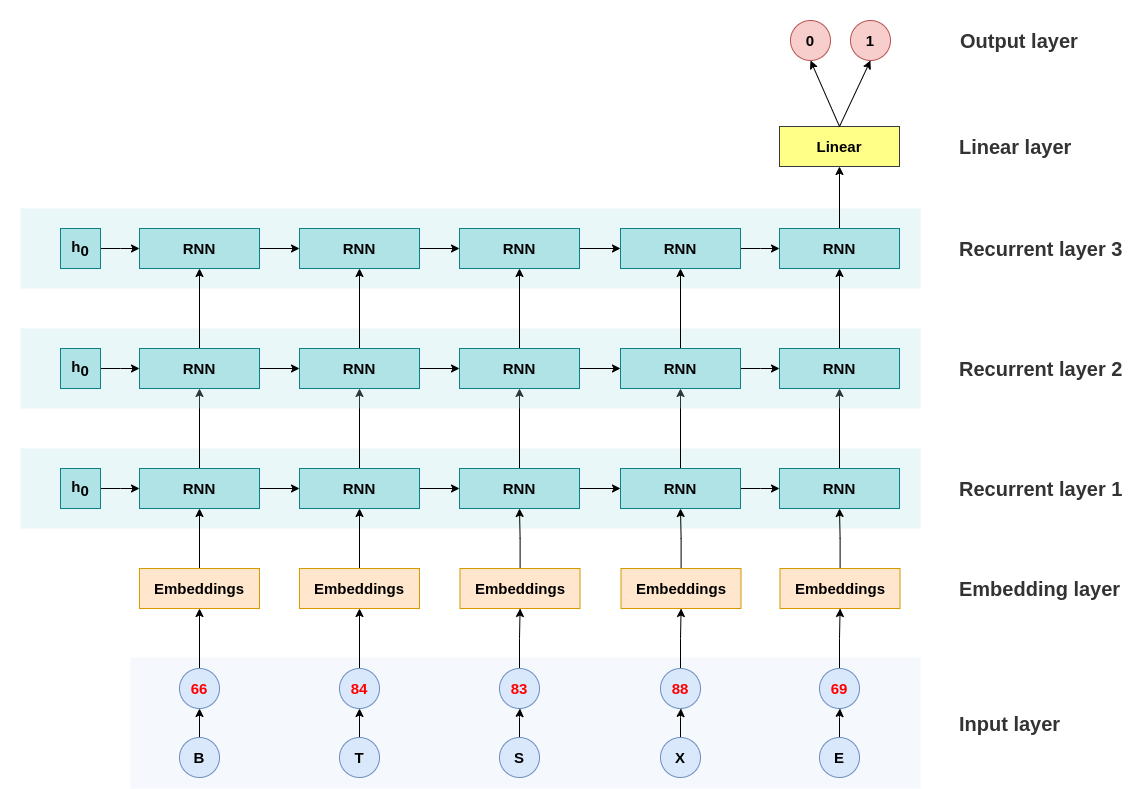
\includegraphics[width=0.85\linewidth]{images/experiments/training_rnn.png}
	\caption[Training recurrent networks]%
	{Visualizing training of a recurrent network with 3 recurrent layers, each layer consisting of 50 neurons.}
	\label{fig:training_rnn}
\end{figure}

Our base model starts with an input layer that feeds data to the model. Since our data is in text format, we convert each character into its corresponding ASCII value. This conversion is visualized in figure \ref{fig:training_rnn} with a valid example Reber sequence, \textbf{BTSXE}. Furthermore, we are working with batches, so all the sequences in a batch must be of equal length. Therefore, we apply zero-padding to ensure all the sequences in a given batch are of the same length.

After the input layer, the second layer is an embedding layer that transforms each input character into a fixed-length vector as visualized in figure \ref{fig:input-to-embedding}. In our case, this embedding layer is of shape $(128, 50)$, where $128$ is the number of possible ASCII characters, and $50$ is the size of each embedding vector known as embedding dimensions. The value of an embedding dimension must be equal to the number of neurons in the next layer.

\begin{figure}[h]
	\centering
	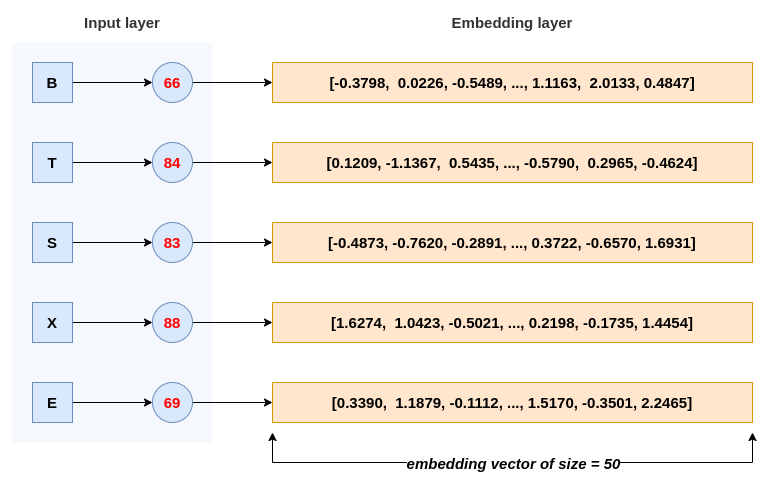
\includegraphics[width=0.85\linewidth]{images/experiments/input-to-embedding.png}
	\caption[Generating embeddings of example input sequence]%
	{Generating embeddings of example Reber sequence after converting each character of this sequence into its corresponding ASCII value.}
	\label{fig:input-to-embedding}
\end{figure}

After the embedding layer, the subsequent three layers are recurrent, each layer containing $50$ neurons. These layers start with an initial hidden state of shape \textit{(batch size, hidden size)}, comprising all zeros. In LSTM, these layers begin with one initial hidden state and one initial cell state, both of similar shape and comprising of all zeros. Each neuron in recurrent layers is an individual RNN unit with either Tanh or ReLU nonlinearity in case of vanilla recurrent network, LSTM unit in case of LSTM recurrent network and GRU unit in case of GRU recurrent network as visualized in the following figure:

\begin{figure}[h]
	\centering
	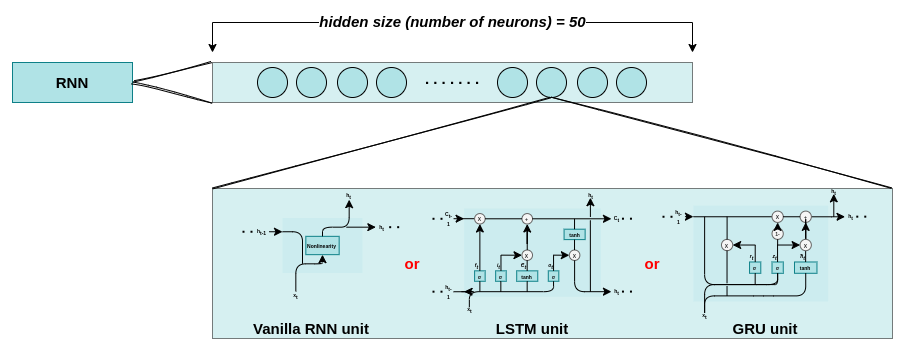
\includegraphics[width=1.0\linewidth]{images/experiments/recurrent_layer.png}
	\caption[Visualization of a single recurrent layer]%
	{Visualizing a single recurrent layer from our model (fig. \ref{fig:training_rnn}). Each neuron is either an individual RNN unit (fig. \ref{fig:rnn_unit}) or an LSTM unit (fig. \ref{fig:lstm_unit}), or a GRU unit (fig. \ref{fig:gru_unit}).}
	\label{fig:recurrent_layer}
\end{figure}

These recurrent layers are followed by a linear layer that takes input from the third recurrent layer and applies the following linear transformation on the input:
\begin{equation}
\label{eq:linear}
    \hat{y} = xW^{T}+b
\end{equation}
where $\hat{y}$ is the output, $W$ represents weight matrices of shape $(output\_size=2, input\_size=50)$, $x$ is the input, and $b$ is bias of shape $(output\_size=2)$.

Since the third recurrent layer's hidden size is $50$, the linear layer's input is of size $50$, and output is of size two because our target has only two classes, $\{0, 1\}$, as shown in figure \ref{fig:output_layer}.

\begin{figure}[h]
	\centering
	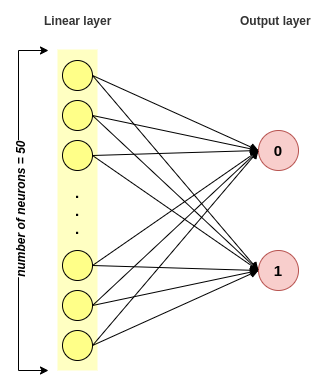
\includegraphics[width=0.3\linewidth]{images/experiments/output_layer.png}
	\caption[Visualization of linear layer's connection to output layer]%
	{\textbf{Visualizing of linear layer's connection to output layer.} Each of the 50 neurons from the linear layer is densely connected to both the output layer neurons.}
	\label{fig:output_layer}
\end{figure}

For our example Reber sequence, the final output is in the form of a float array of size two, for instance, $[-0.8169, 1.3229]$. To transform it into $0$ or $1$, take the index of maximum value from this array. After getting an output, the model calculates the cross-entropy loss and optimizes it via backpropagation through time to a minimum value to achieve better performance.

We train this model on our training dataset of $18750$ sequences for $50$ epochs, and to check its performance, we evaluate it on the test dataset of $6250$ sequences. This training and evaluation employ the hyper-parameters shown in the following table.

\begin{table}[h]
	\centering
	\begin{tabular}{|c|c|}
	    \hline
		\textbf{Hyper-parameter} & \textbf{Value} \\
		\hline
		Learning rate & 0.001 \\
		Loss & Cross-Entropy Loss \\
		Optimizer & Adam \\
		Batch size & 32 \\
		\hline
	\end{tabular}
	\caption[Hyper-parameters used for training and evaluating the base model]{Hyper-parameters used for training and evaluating the base model.}
	\label{tab:hype_param_base}
\end{table}

Since we work with four different RNN variants, namely RNN with Tanh nonlinearity, RNN with ReLU nonlinearity, LSTM, and GRU, we also perform this training four times.

As we have already established, training a recurrent network is computationally expensive and time-consuming. Therefore all four models in our experiment are trained on a Tesla K80 GPU.

% -----------------------------------------------------------------------------------------------------------
% ----------------------------------------------- PRUNE RNNs ------------------------------------------------
% -----------------------------------------------------------------------------------------------------------

\newpage
\section{Pruned Recurrent Neural Networks}\label{section:pruned_rnn}

One of the ways to introduce sparsity in recurrent networks is to prune weight below a certain threshold. As shown in figure \ref{fig:rnn}, we have three different types of weights; input-to-hidden weights, hidden-to-hidden weights, and hidden-to-output weights. In our experiment, we individually and simultaneously prune input-to-hidden and hidden-to-hidden weights as envisioned in the following figure:

\begin{figure}[h]
  \begin{subfigure}{0.33\textwidth}
    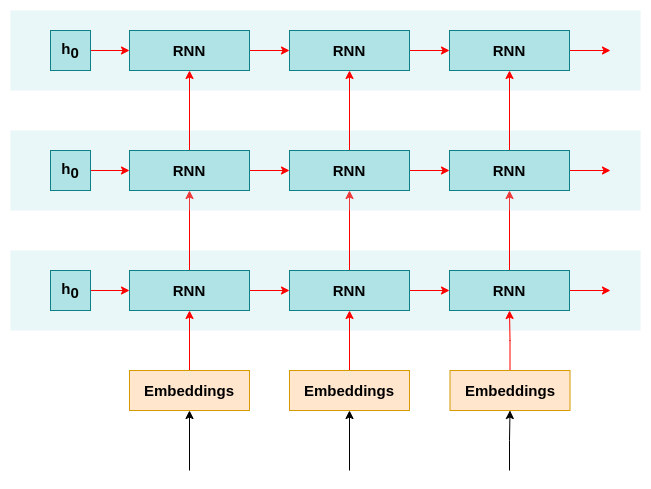
\includegraphics[width=\linewidth]{images/experiments/both_prune.png}
    \caption{} \label{fig:both}
  \end{subfigure}%
  %\hspace*{\fill}   % maximize separation between the subfigures
  \begin{subfigure}{0.33\textwidth}
    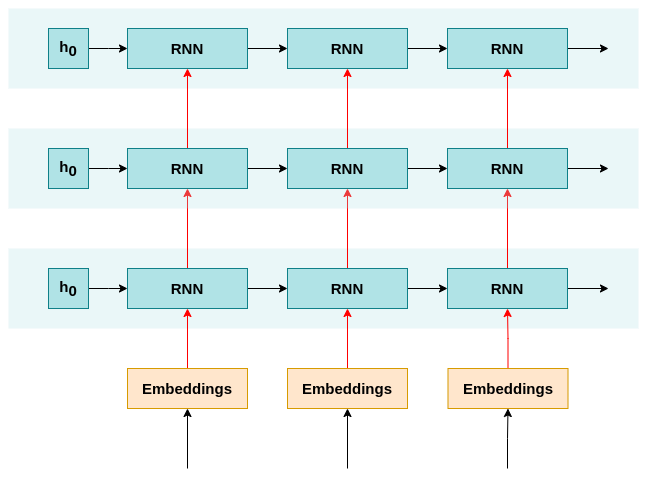
\includegraphics[width=\linewidth]{images/experiments/i2h_prune.png}
    \caption{} \label{fig:i2h}
  \end{subfigure}%
  %\hspace*{\fill}   % maximizeseparation between the subfigures
  \begin{subfigure}{0.33\textwidth}
    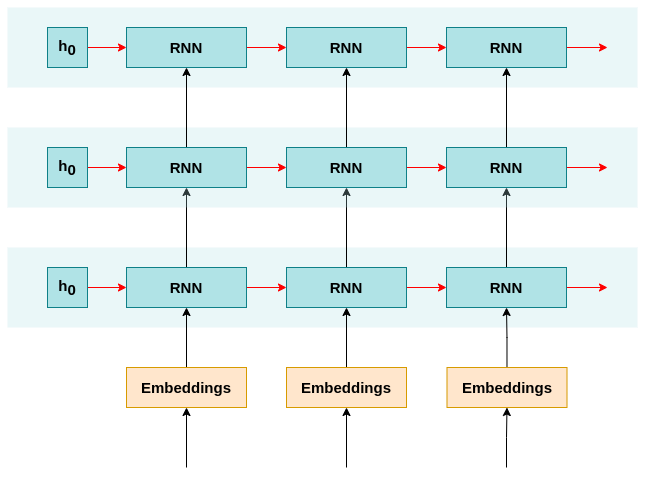
\includegraphics[width=\linewidth]{images/experiments/h2h_prune.png}
    \caption{} \label{fig:h2h}
  \end{subfigure}

\caption[Simultaneous and individual pruning of i2h and h2h weights]{Simultaneously and individually pruning input-to-hidden and hidden-to-hidden weights. The red right arrow (\textcolor{red}{$\longrightarrow$}) resembles the pruning of hidden-to-hidden weight, while the red up-arrow (\textcolor{red}{$\big\uparrow$}) resemble the pruning of input-to-hidden weight. Fig. \ref{fig:both} illustrates pruning both, input-to-hidden and hidden-to-hidden weights, fig. \ref{fig:i2h} illustrates pruning only input-to-hidden weights, and fig. \ref{fig:h2h} illustrates pruning only hidden-to-hidden weights.} \label{fig:pruning}
\end{figure}

The threshold based on which we prune weights is calculated based on the percent of weights to prune. Therefore, for example, to prune $p=10\%$ of weights for a given layer, the threshold is the 10th percentile of all the \textbf{absolute} weights in that layer (code \ref{code:threshold}). In our experiment, as shown in figure \ref{fig:flowchart_pruning}, we go from percent $p=10$ to $100$ while incrementing $p$ by $10$ after each round.

Using this threshold value, we create a binary tensor called a mask, where $1$ corresponds to the \textbf{absolute} weight value above the threshold, and $0$ corresponds to the \textbf{absolute} weight value below the threshold (code \ref{code:mask}) in the corresponding weight matrix. Element-wise multiplication of this binary mask with the corresponding weight matrix zero-outs the absolute weight values below the threshold value.

To understand this binary mask generation and mask multiplication, consider the following example weight matrix of shape $(3, 3)$ with float values between $-1$ and $1$:

\[
\begin{bmatrix}
    -0.685 & 0.530 & -0.464 \\
    -0.534 & 0.828 &  0.045 \\
    -0.123 & 0.629 & -0.014
\end{bmatrix}
\]

This weight matrix corresponds to a linear layer with 3 neurons densely connected to the next linear layer with 3 neurons as shown in the below figure:

\begin{figure}[h]
	\centering
	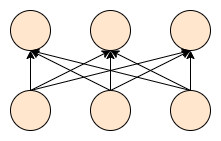
\includegraphics[width=0.3\linewidth]{images/experiments/three_neuron.png}
	\caption[Two densely connected linear layers]%
	{Two densely connected linear layers, each layer containing 3 neurons. This visualization corresponds to the example weight matrix shown above.}
	\label{fig:three_neuron}
\end{figure}

To prune $10\%$ percent of weight values from the above matrix, we calculate the threshold by finding the 10th percentile of this matrix's \textbf{absolute} values, which is $0.0387$. Using this threshold, we create a binary mask of shape $(3, 3)$, where values at positions that correspond to the below threshold \textbf{absolute} values in the weight matrix are kept $0$ while other values are kept $1$ as shown below:

\[
\begin{bmatrix}
    -0.685 & 0.530 & -0.464 \\
    -0.534 & 0.828 &  0.045 \\
    -0.123 & 0.629 & \textcolor{red}{-0.014}
\end{bmatrix}
\longrightarrow
\begin{bmatrix}
    1 & 1 & 1 \\
    1 & 1 &  1 \\
    1 & 1 & \textcolor{red}{0}
\end{bmatrix}
\]

By performing element-wise multiplication of this binary mask with our weight matrix, we get a pruned weight matrix as shown below:

\[
\begin{bmatrix}
    -0.685 & 0.530 & -0.464 \\
    -0.534 & 0.828 &  0.045 \\
    -0.123 & 0.629 & \textcolor{red}{-0.014}
\end{bmatrix}
\circ
\begin{bmatrix}
    1 & 1 & 1 \\
    1 & 1 &  1 \\
    1 & 1 & \textcolor{red}{0}
\end{bmatrix}
=
\begin{bmatrix}
    -0.685 & 0.530 & -0.464 \\
    -0.534 & 0.828 &  0.045 \\
    -0.123 & 0.629 & \textcolor{red}{0}
\end{bmatrix}
\]

The value $0$ in this weight matrix represents the missing connections between the third neuron of the first and second linear layer. After applying the mask, the simple neural network shown in the figure \ref{fig:three_neuron} looks like below:

\begin{figure}[h]
	\centering
	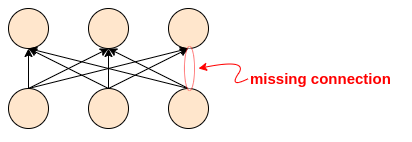
\includegraphics[width=0.5\linewidth]{images/experiments/pruned_three_neuron.png}
	\caption[Two densely connected linear layers after pruning]%
	{Two densely connected linear layers containing 3 neurons show the absence of connection between each layer's third neuron after pruning. This visualization corresponds to the pruned weight matrix.}
	\label{fig:pruned_three_neuron}
\end{figure}

We follow a similar mask generation approach and element-wise multiplication for each corresponding weight matrix in each recurrent layer of our trained model. As shown above, this pruning process returns a pruned weight matrix for each corresponding weight matrix. After pruning, we evaluate pruned model's performance on the test dataset to see how such pruning affects an already trained model's overall accuracy.

Once we have the pruned model's performance, the next step is to retrain the same pruned model to estimate the number of epochs required to regain the accuracy. We use the same pruned weight matrices throughout the entire retraining course. This helps us understand how long it takes for a recurrent network to relearn and update weight matrices to make up for the lost connections.

These pruning and retraining steps are repeated three times per RNN variant (i.e., RNN-Tanh, RNN-ReLU, LSTM, and GRU), first time for pruning both, input-to-hidden and hidden-to-hidden weights, the second time for pruning only input-to-hidden weights, and the third time for pruning only hidden-to-hidden weights. 

% -----------------------------------------------------------------------------------------------------------
% ----------------------------------------------- RA-ST RNNs ------------------------------------------------
% -----------------------------------------------------------------------------------------------------------

\newpage
\section{Randomly Structured Recurrent Neural Networks}\label{section:random_rnn}

The pruning method to induce sparsity in a recurrent network works by canceling connections between neurons of two separate layers. While in this section, we explain another method to induce sparsity by generating random structures that are already sparse. This method was introduced for Artificial Neural Network by Stier et al. in \cite{julian}, which we will revise to make it suitable for our goal.

The first step of this experiment is to generate random graphs irrespective of how they might correspond to a neural network. We generate $100$ connected Watts–Strogatz (\ref{subsubsection:wsmodel}) and Barabási–Albert (\ref{subsubsection:bamodel}) graphs using the graph generators provided by the networkx\footnote{NetworkX is an open-source Python library that empowers users to create and manipulate various graph structures.}. Each of these graphs contains nodes between $(10, 51)$, meaning the corresponding neural architecture will have $(10, 51)$ neurons.

The networkx graph generators return undirected graphs. Therefore, the next is to make them directed. Converting a random graph into a Directed Acyclic Graph is vital to make it easier to compute layer indexing.

After converting a random graph into a DAG, the next step is to compute layer indexing of all the nodes in this DAG. This helps us identify which node of this DAG belongs to which layer in the resulting neural network. The recursive algorithm to compute layer indexing of a node (similar to the one used by Stier et al. in \cite{julian}) is as below:

\begin{algorithm}
  \DontPrintSemicolon
  \caption[Compute layer indexing of nodes]%
  {Recursive function to compute layer indexing of nodes}
  \label{alg:layer_index}
  
    \KwIn{Graph $G$, Set of nodes $V$, Set of edges $E$}    
    \KwOut{Layer index mapping for each node $v \in V$}
  
    \SetKwFunction{func}{LayerIndexOf}
    \SetKwProg{Fn}{Def}{:}{}
    
    \Fn{\func{$v$}}{
        $l \gets [-1]$ \tcp*{List $l$, initialized with an element $-1$}
        
        \ForEach{$s \in V | E_{s \rightarrow v}$}{
            $l$.append(LayerIndexOf($s$))
        }
        
        \textbf{return} (max($l$) + 1)
    }
    
    $indexes \gets dict()$ \tcp*{Initializing an empty dictionary, $indexes$}
    \ForEach{$v \in V$}{
        $indexes[v] \gets $ LayerIndexOf($v$)
    }
\end{algorithm}

This recursive function outputs layer indexing of all nodes in our DAG, based on which we generate our final neural architecture, which then we convert into a recurrent network by introducing hidden-to-hidden connections, i.e., recurrent connections.

Once we have our randomly structured recurrent network, the final step is to embed it between an embedding layer and a linear layer. The embedding layer transforms data from the input layer into a fixed-length vector and feeds them to our recurrent layer. The linear layer takes the last recurrent layer's output, applies a linear transformation shown in equation \ref{eq:linear}, and generates final outputs.

\subsection{From Random Graph to recurrent network: An example}

To begin, consider the following undirected graph containing 5 nodes:

\begin{figure}[h]
	\centering
	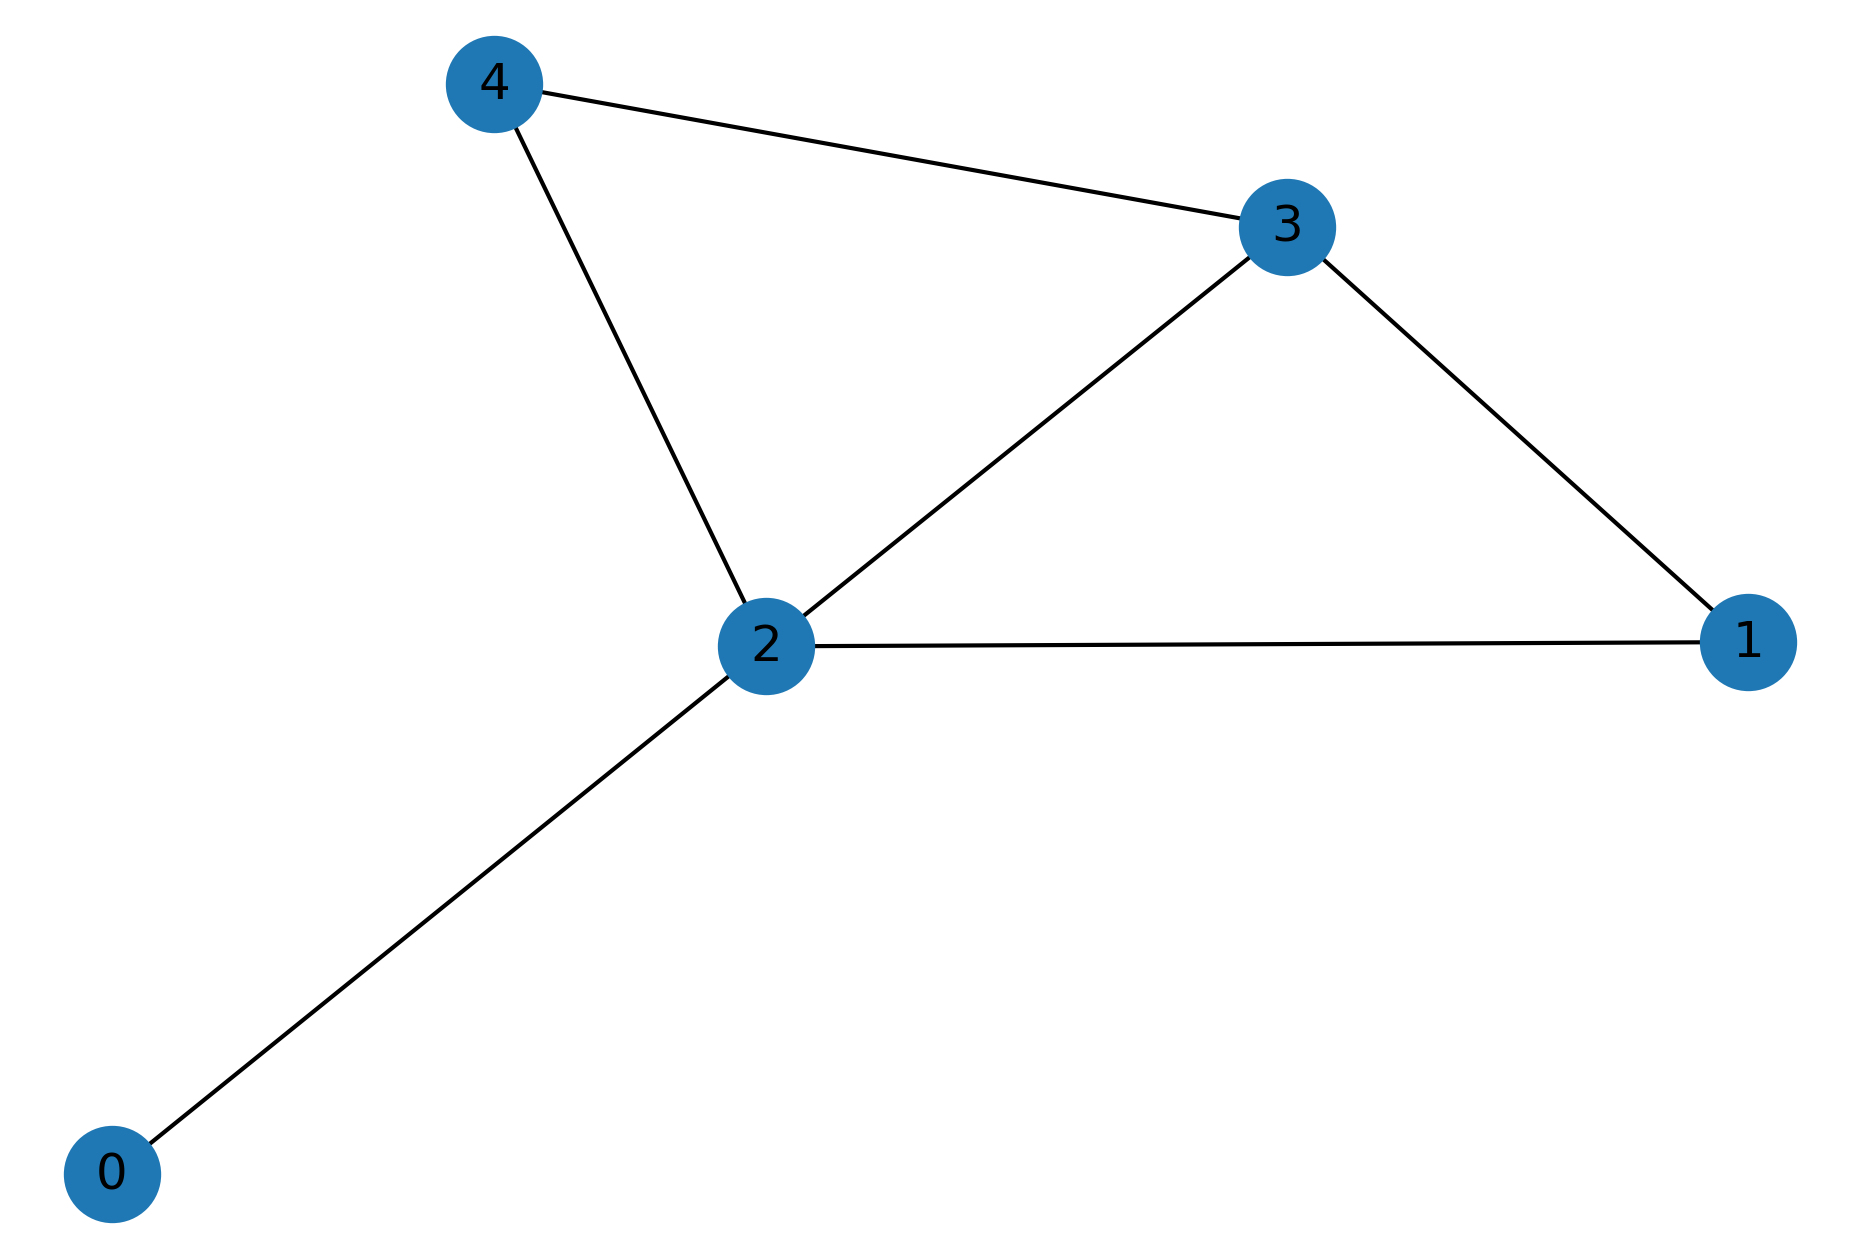
\includegraphics[width=0.45\linewidth]{images/experiments/undirected.png}
	\caption[Undirected graph containing $5$ nodes]%
	{An undirected graph containing $5$ nodes.}
	\label{fig:undirected}
\end{figure}

The next step is to convert this graph into a DAG. This conversion introduces directed edges from one node to another, as shown below:

\begin{figure}[h]
	\centering
	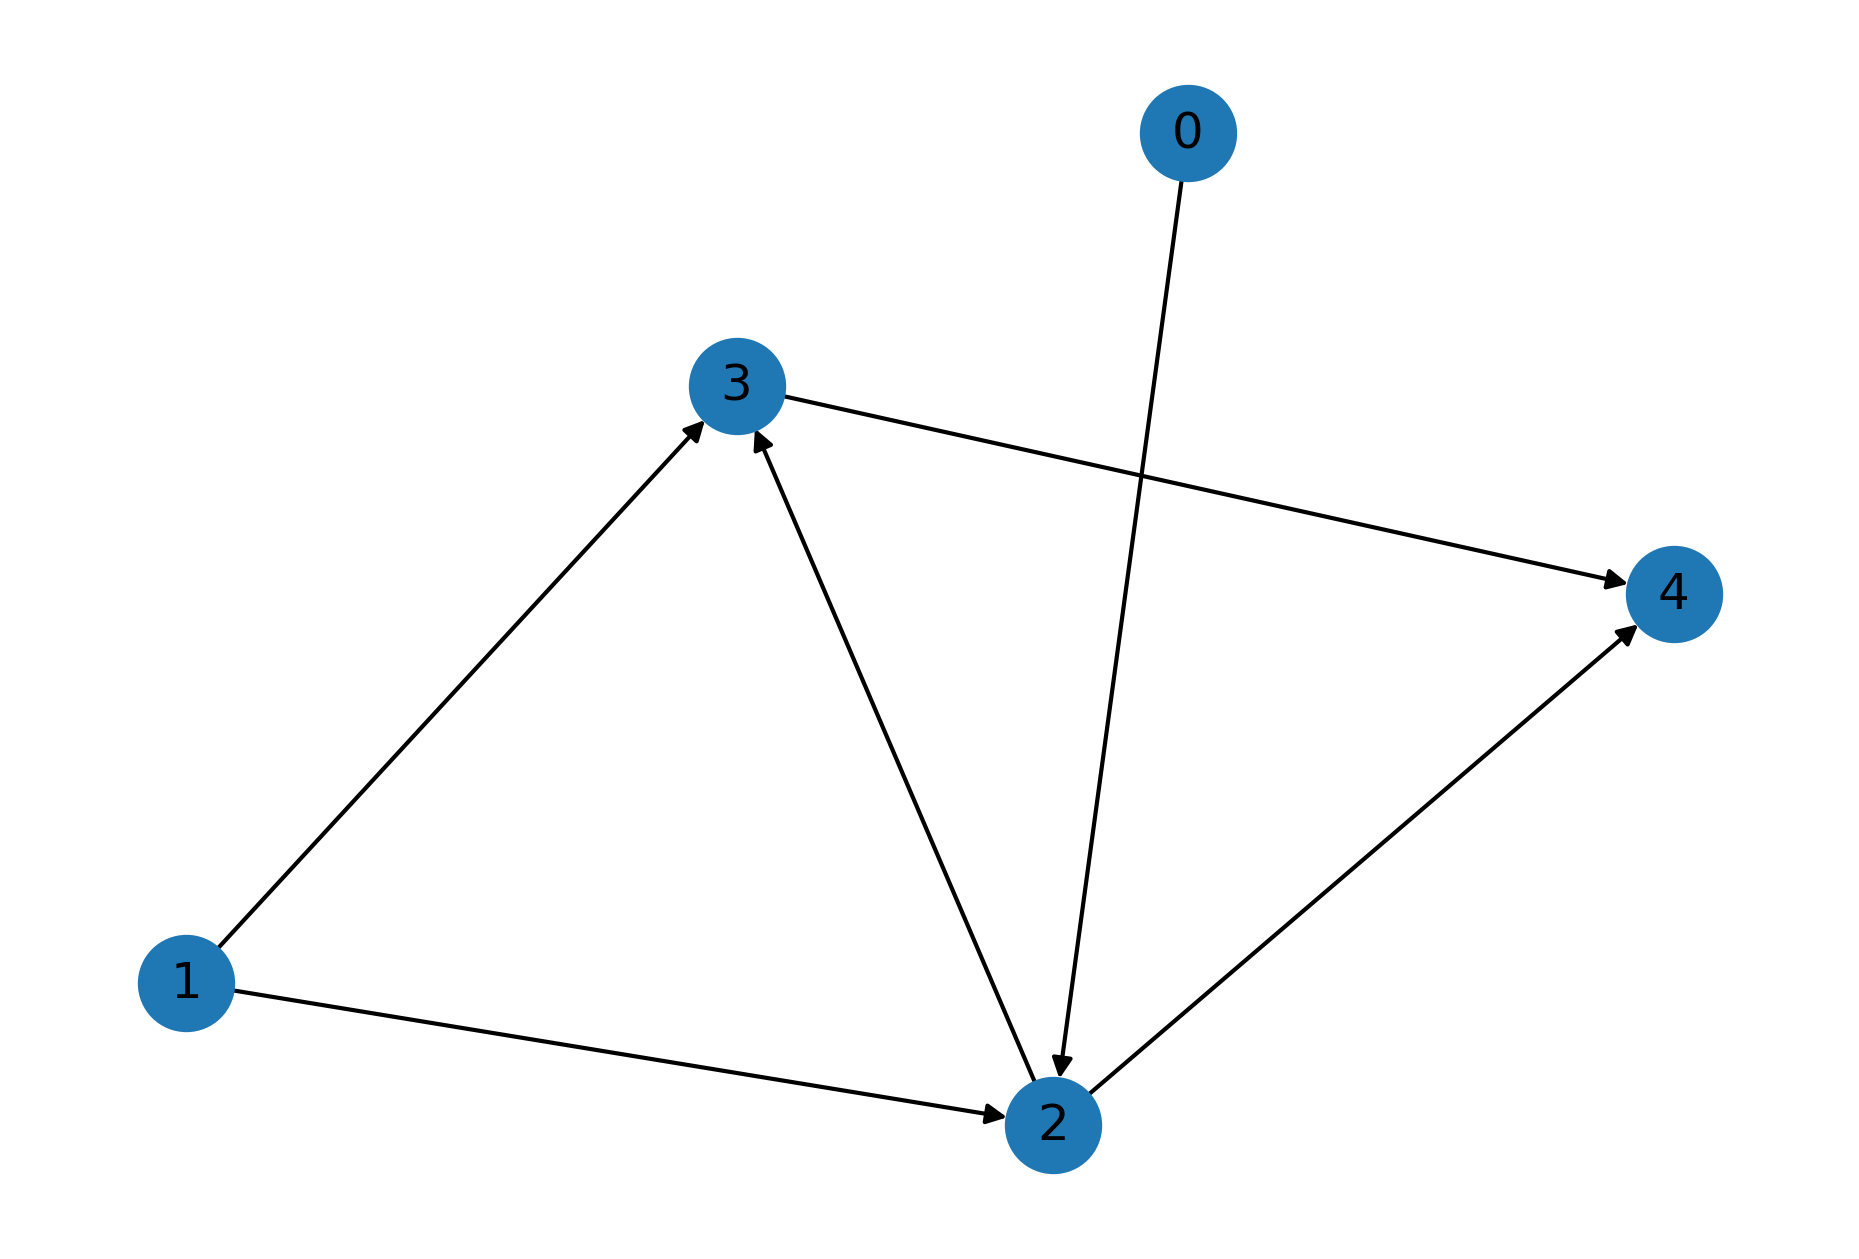
\includegraphics[width=0.45\linewidth]{images/experiments/directed.png}
	\caption[Directed graph containing $5$ nodes]%
	{A directed graph containing $5$ nodes.}
	\label{fig:directed}
\end{figure}

The next step is to compute layer indexing of all $5$ nodes in this DAG using algorithm \ref{alg:layer_index}. The following table shows the values of important variables in this algorithm and the final layer indexing:

\begin{table}[h]
	\centering
	\begin{tabular}{|c|c|c|c|}
	    \hline
		\textbf{Node $v$} & \textbf{Set of $s, \forall s \in V | E_{s \rightarrow v}$} & List $l$ & Layer index of node $v$\\
		\hline
		0 & \{\} & [-1] & 0\\
		1 & \{\} & [-1] & 0\\
		2 & \{0, 1\} & [-1, 0, 0] & 1\\
		3 & \{1, 2\} & [-1, 0, 1] & 2\\
		4 & \{2, 3\} & [-1, 1, 2] & 3\\
		\hline
	\end{tabular}
	\caption[Computing layer indexing of example DAG]{We first identify a set of all the parent nodes for a given node $v$, then append layer indexing of these parent nodes to the list $l$, and finally return $max(l) + 1$ as layer index of node $v$.}
	\label{tab:layer_index}
\end{table}

The next step is to create a neural architecture using this layer indexing:

\begin{figure}[h]
	\centering
	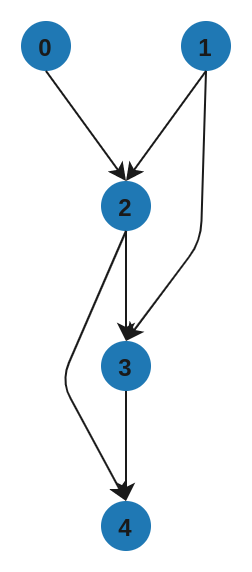
\includegraphics[width=0.25\linewidth]{images/experiments/neural_arc.png}
	\caption[Neural architecture generated using the layer indexing]%
	{A neural architecture of $4$ layers, generated using the layer indexing of nodes shown in table \ref{tab:layer_index}.}
	\label{fig:neural_arc}
\end{figure}

Once we have the neural architecture, as shown in figure \ref{fig:neural_arc}, the next step is to introduce recurrent connections. This will give us our randomly structured recurrent network.

Attaching this randomly structured recurrent network between an embedding layer and a linear layer, as shown in the below figure, gives us our final model:

\begin{figure}[h]
	\centering
	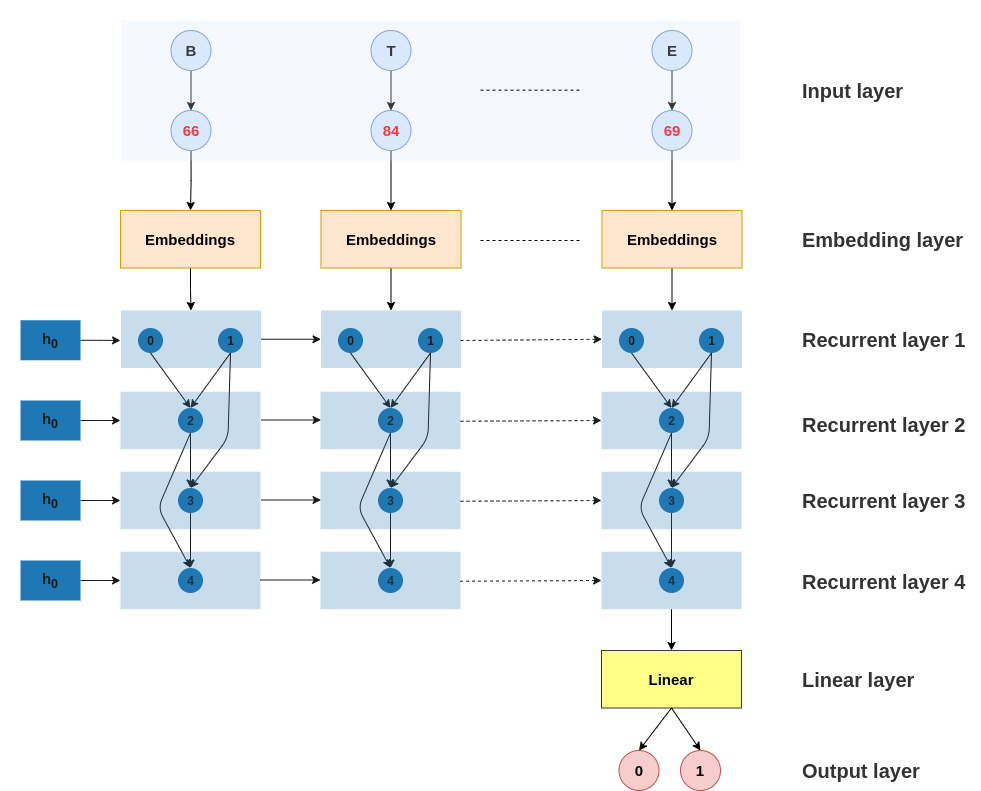
\includegraphics[width=0.8\linewidth]{images/experiments/recurrent_arc.png}
	\caption[Complete model with recurrent architecture generated from a random graph]%
	{A complete trainable model with an input and output layer, an embedding layer, a linear layer, and a recurrent architecture generated from a random graph.}
	\label{fig:recurrent_arc}
\end{figure}

This is the final trainable model that we train on our training dataset for $15$ epochs and evaluate on the test dataset.

Similarly, we generate $200$ random graphs with nodes between $(10, 51)$ for each RNN variant (i.e., RNN-Tanh, RNN-ReLU, LSTM, and GRU), convert them into a recurrent network, and create the full model for each randomly structured recurrent network, as shown in figure \ref{fig:recurrent_arc}. We train them on our train dataset for $15$ epochs with hyper-parameters shown in table \ref{tab:hype_param_base} except with batch size of $128$. Finally, we evaluate them on our test dataset and store the performance that is useful in the next part of the experiment.

\subsection{Identifying important graph properties}

While training random structure recurrent networks, we also record specific graph properties (mentioned in section \ref{subsection:properties}) of its base random graph. After training and evaluation are complete, we store its accuracy, creating a small dataset of $200$ rows.

Since the graph properties in our small dataset are in different ranges, we apply MinMax scaler on our dataset to scale each graph property between a range $(0, 1)$.

Next, we split this dataset into a train-test with a $0.9/0.1$ ratio. We train three different regressor algorithms: Bayesian ridge regressor, Random Forest regressor, and Ada Boost regressor, on the train set with graph properties as features and its corresponding accuracy as the target.

Then, we evaluate each regressor algorithm on the test set and report an R-squared value to understand how our data fit each regressor model.

This chapter described our experiments with Sparse RNN in detail. After getting familiarized with our experiments, we present our experiments' results and their corresponding visualizations in the next chapter.